%!TEX root = report.tex


\section{Experiments}
We implement our model in Section \ref{Sec:methodology} with TensorFlow, 
and apply our code on the dataset described in Section \ref{Sec:ProblemData}. 
To be specific, we train and tune our model on the 2013 Train and Dev dataset, 
and evaluate our model on the Test 2013--2015 dataset. The focus of this section 
is to compare our author activated CNN model performance with the baseline CNN model.

\subsection{Experiment Setting}
We employ the pretrained word embeddings by Austudillo et al.\ [13]. 
These embeddings are obtained via training on a corpus of 52 million tweets
using the structure skip-gram model [14], and have been shown to
perform very well on sentiment analysis tasks [1].
We also use the same evaluation metric as the SemEval challenge.

We pretrain the word embedding using several existing network node embedding methods 
including DeepWalk [2], LINE [3], 
and node2vec [4]. These methods are applied to all the FOLLOWER+,
MENTION+, and RETWEET+ networks. In addition, to provide a baseline for different node embedding methods, 
we use purely random node vector.



Regarding baseline models, we adopt the state-of-the-art convolutional neural network model
methodology for sentiment analysis. This model is the basis model of our Author Activation CNN Model and
has been described in Section \ref{Sec:methodology}. As a second baseline model, we adopt
the Social Attention model [1] which models the soft-assignment of users to communities. 


\paragraph{Parameter tuning} 
For both the baseline CNN model and author activated CNN model, we tune all the hyper parameters 
on the SemEval 2013 Dev dataset, including
\begin{itemize}
\item number of bigram filters for the CNN models, from \{16, 32, 50, 100\};
\item dropout rate, from \{0.1, 0.2, 0.4\};
\item $L_2$-penalty coefficient, from \{1e-6, 1e-4, 1e-2\};
\item author embedding dimension, from \{16, 32, 50, 100\}.
\end{itemize}
Moreover, we precomputed the author embeddings on all the FOLLOWER+,
MENTION+, and RETWEET+ networks with three node embedding methods. Using different networks
as well as embedding algorithms can all be considered as hyper parameters.
We also adopted early stopping method based on Dev Performance to prevent our model from overfitting.

For the Social Attention model, we use the best hyper parameter set provided by the author [1].


\subsection{Results}
\begin{table}[tbp]
\begin{center}
\begin{tabular}{|c|c| c | c c c |}
\hline
 & CNN & SA
\footnotemark
& DeepWalk & LINE & node2vec\\
\hline
Dev2013  & 68.85 &69.52 & 67.71 & 69.51 & 68.58 \\
\hline
Test2013  & 69.53 & 69.98& 67.58 & 69.67 & 68.58 \\
Test2014  & 72.41 & 72.70 & 71.46 & 71.44 & 71.46 \\
Test2015  & 64.40 &65.28 & 64.71 & 64.57 & 64.25 \\
\hline
Avg test sets & 68.78 &69.32& 67.92 & 68.56  & 68.10 \\
\hline
\end{tabular}
\end{center}
\caption{Prediction performance on each Dev and Test Sets. }
\label{Tb:Results}
\end{table}%
\footnotetext{Social Attention model [1]. Note that even after contacting the authors and obtaining their code, 
we still fail to retrieve their declared result in the paper. Here we put the implemented result using their provided code.} 



Table \ref{Tb:Results} summarizes the empirical result of our experiments. Both baseline CNN model 
and our author activated CNN model are tuned for all parameters The best hyper parameter sets for baseline 
CNN model is 100 bigram filters, 0.4 dropout rate, and 1e-2 for $L_2$ penalty coefficient. The best 
hyper parameter sets for the author activated CNN model is 100 bigram filters, 100 author embedding dimension, 
and from RETWEET+ network. The best dropout rate and $L_2$ penalty coefficient depends on which 
node embedding method we use. From the table, we see that the improvement after adding the node 
embedding is insignificant. The author-activated CNN model sometimes do even worse in terms of test 
sets prediction. Different node embedding scheme does not seems to have big impact on the downstream 
prediction task.





\subsection{A two-stage training method}
We believe the reason for unsatisfying result is that author informations are considered too early 
in our training process. We combine author information to solve the problem of language variation. 
However, immediately after we randomly initialize the weights in baseline CNN model, language variation 
can not be seen, i.e., we are not more likely to make wrong prediction to twitter between a pair of friends. 
At this time, most gains are achieve by training the sentence interpretation part (encoded by baseline CNN model)
rather than solving language variation. Therefore, the update on author embedding weights are almost purely 
random thus will harm our model in the long run. The language variation is better heard after the sentence 
interpretation part is mature. In the training process, this is the time when the baseline CNN model start to overfit. 

Therefore, we propose a two-stage training method.
In the first stage, we fix the weights related with author embedding, and only train the weights existing in the
baseline CNN model. After several epochs of training, the improvement of development set prediction 
performance starts to fluctuate  (See Figure \ref{Fig:TwoStage}), we interpret this an a sign of baseline 
CNN model overfitting, and it is only at this stage, the second stage, that we start to train the layer related with
author embedding. 

Table \ref{Fig:TwoStage} demonstrates the performance of two-stage training method. We consider two variations. 
First, in the second stage we update the weight matrices in both sentence convolution layer and author embedding
processing layer. Second, in the second stage, we fix the sentence convolution layer and only update the author embedding
layer. Unfortunately, in both variation, the improvement in prediction performance from adding author embedding
information is not significant. In the first variation (left plot of Figure \ref{Fig:TwoStage}) the prediction performance 
still fluctuate just like the CNN training method; in the second variation, there seems to be no improvement. 


\begin{figure}[tbp] %  figure placement: here, top, bottom, or page
   \centering
\begin{minipage}{0.5\linewidth}\centering
   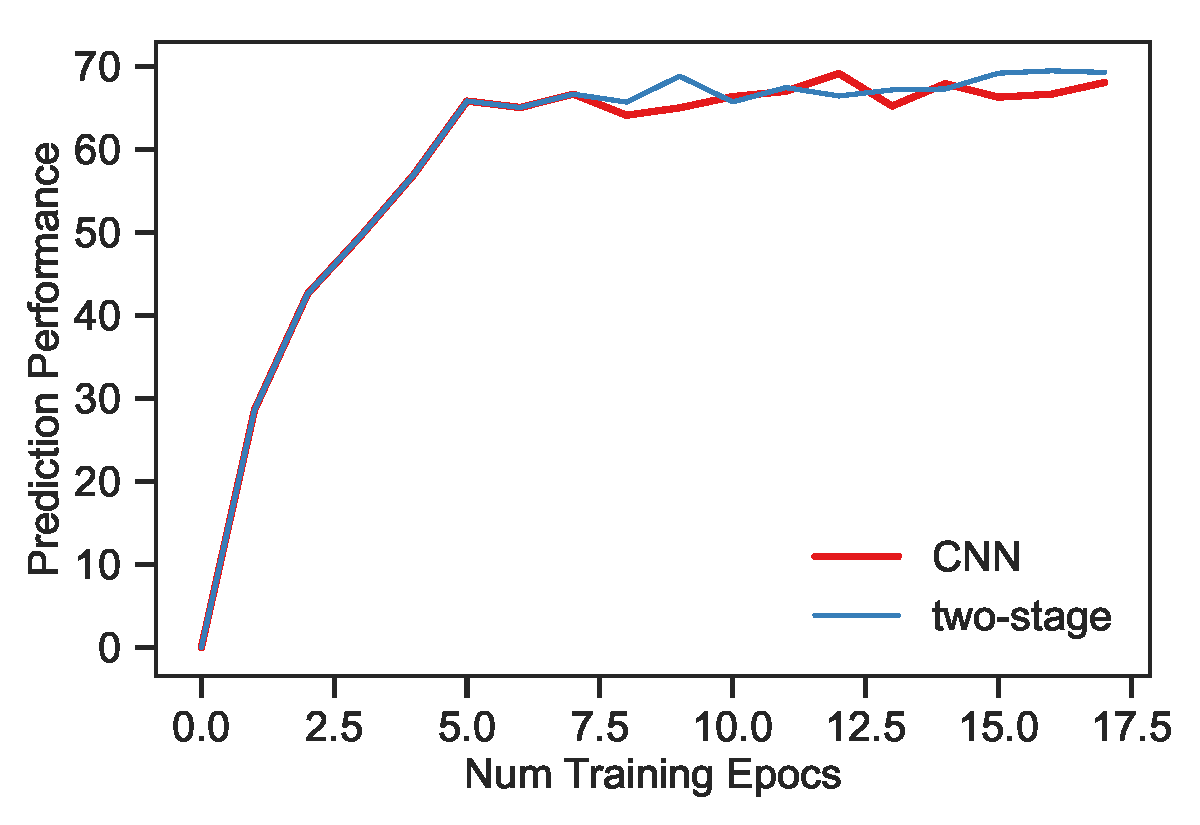
\includegraphics[width=2.5in]{two-stage.pdf} 
   \\{\footnotesize Updating both convolution layer weights and author layer weights   }
\end{minipage}
\begin{minipage}{0.49\linewidth}\centering
   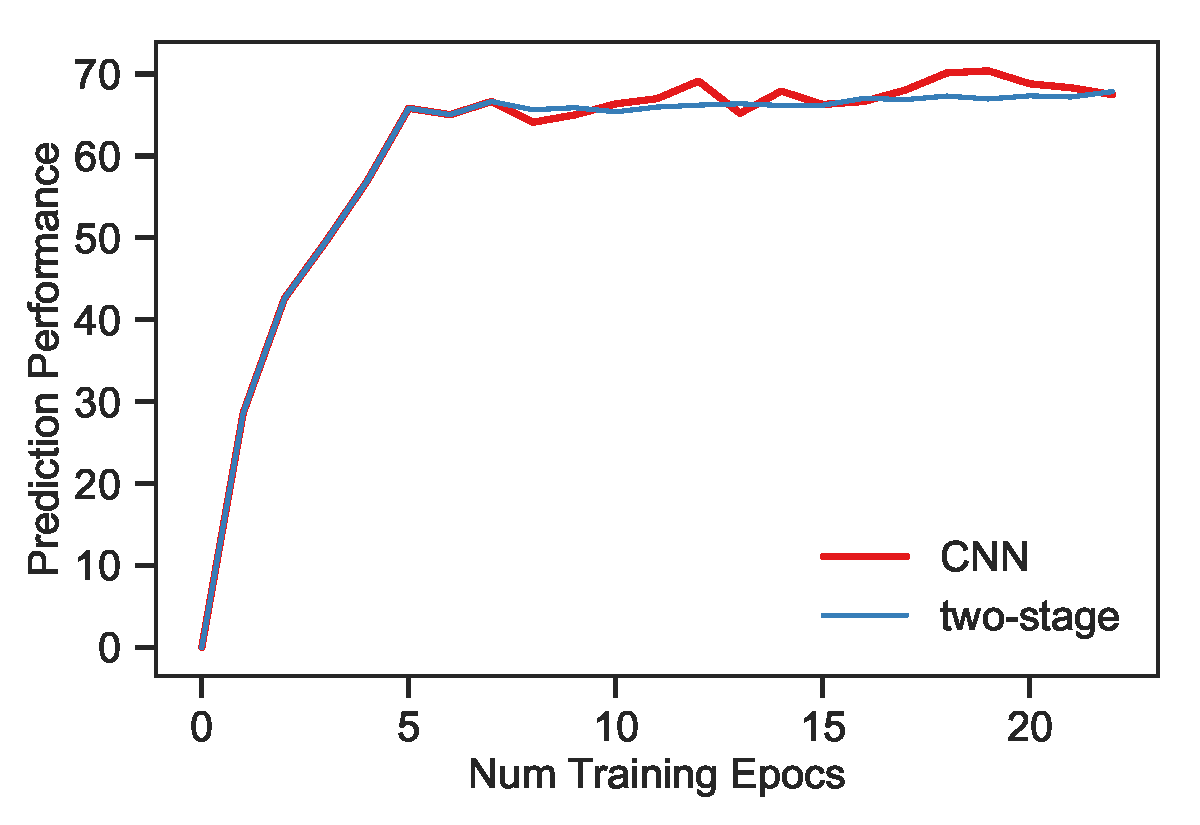
\includegraphics[width=2.5in]{two-stage-fix.pdf} 
   \\{\footnotesize Fix convolution layer and only train author layer weights   }
\end{minipage}
\caption{Performance of two-stage training method.}
\label{Fig:TwoStage}
\end{figure}